\begin{frame}
	\frametitle{Particle Unbinding}
	
%	In general, one can assign every particle a total energy $E$. A particle is considered to be ``bound'' if:
%	\begin{align*}
%		E< 0
%	\end{align*}
%	
%	Considering each clump as an isolated, time independent spherical system of collisionless dark matter particles.
%	
%	In such a system the energy $E_i$ of a particle $i$ in the centre of mass frame of the clump it belongs to can be expressed as 

	In an isolated system in the centre of mass frame, each particle $i$ can be assigned an energy $E_i$:
	\begin{align*}
	E_i = T_i + V_i = \frac{1}{2} m_i \cdot v^2_i + m_i \phi (\vec{r}_i)
	\end{align*}
	
	A particle is considered bound if:
	\begin{align*}
	E_i < 0 \quad \Leftrightarrow \quad v_i < \sqrt{- 2 \cdot \phi(\vec{r}_i)}
	\end{align*}
	
\end{frame}










\begin{frame}
	\frametitle{Particle Unbinding}
	The only considered potential $\phi$ is the gravitational potential of the particles themselves. The potential is determined by the Poisson equation:
	\begin{align*}
		\Delta \phi = 4 \pi G \rho
	\end{align*}
	
	The spherically symmetric Poisson equation  can be solved analytically for $\phi$:
	%
	\begin{align*}
	\phi (r_i) &=  - G \int\limits_{r_i}^{r_{max}} \frac{M(<\tilde{r})}{\tilde{r}^2} \mathrm{d}\tilde{r}
	- G  \frac{M_{tot}}{r_{max}}
	\end{align*}
	%
	Where $M(<r) \equiv \int\limits_0^r 4 \pi \rho(\tilde{r})\tilde{r}^2 \mathrm{d}\tilde{r} $ is the mass enclosed by a sphere of radius $r$ such that the clump's total mass is enclosed by the radius $r_{max}$: $M_{tot} = M(<r_{max})$ and $G$ is the gravitational constant and $\rho$ is the density.
\end{frame}



\begin{frame}
	\frametitle{Results: \dt-dataset}
	
	\begin{tabular}{c c}
		\phewon\ 	& \simple \\[1.5em]
		%
		%	 
		{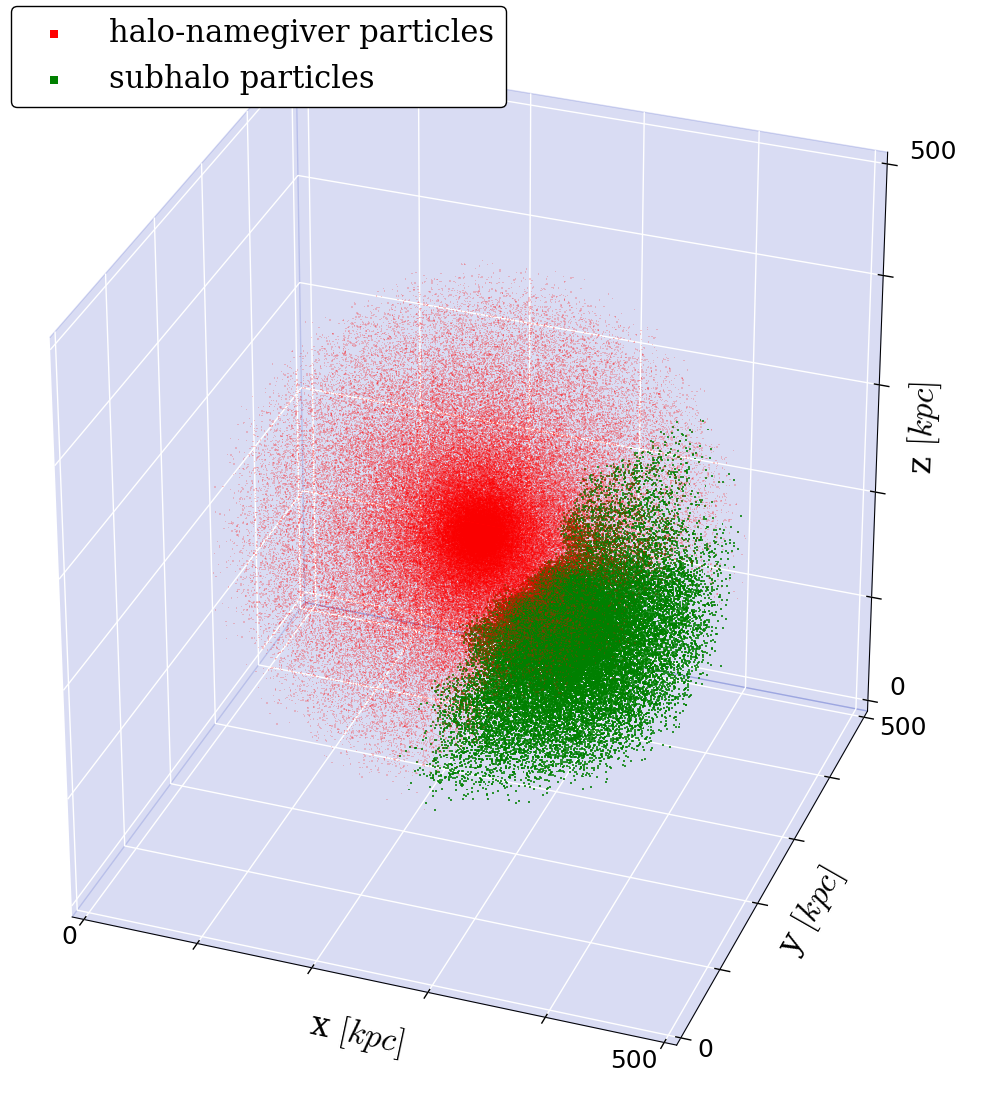
\includegraphics[width = .49\textwidth]{../report/images/dice-two/dice-two-plot-halo1451-phew.png}} \hspace*{-1em} 	& 
		{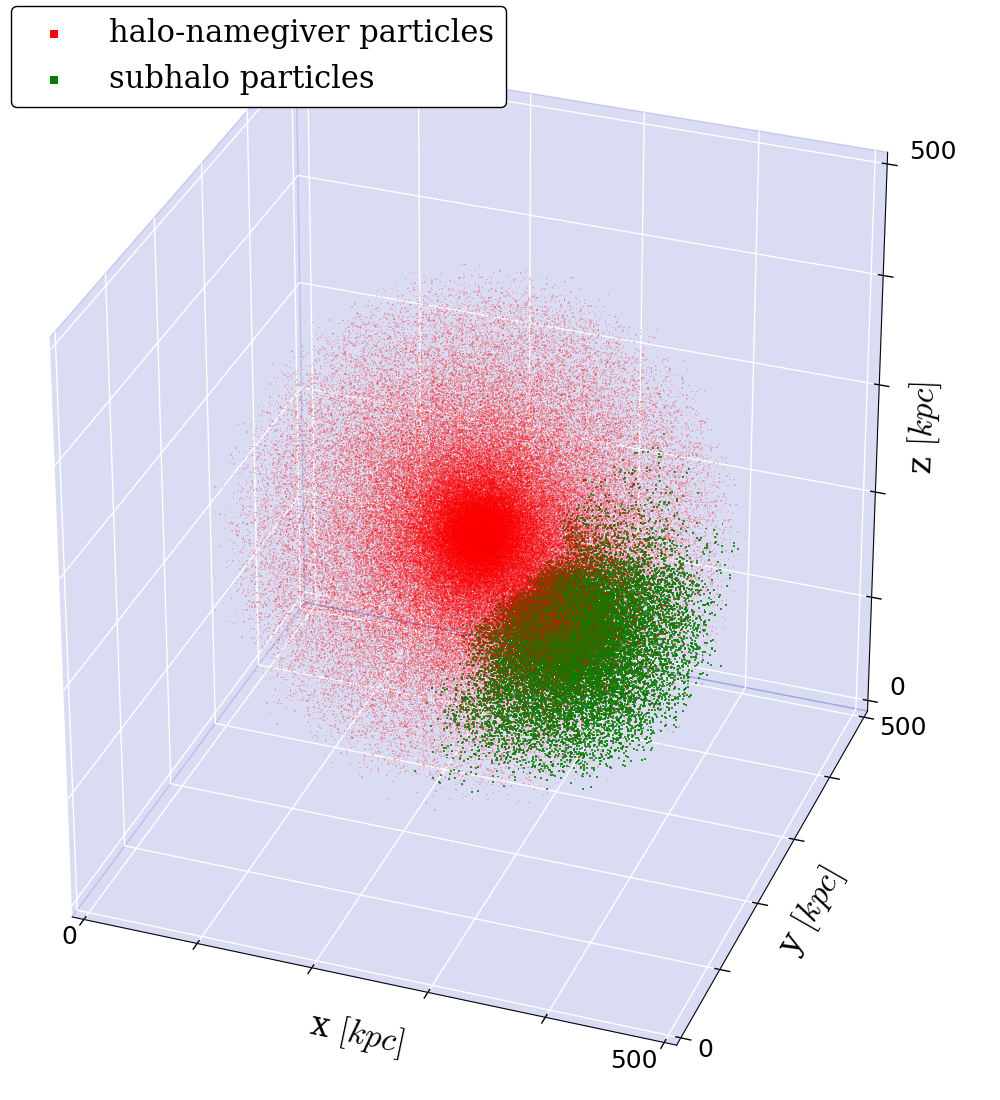
\includegraphics[width = .49\textwidth]{../report/images/dice-two/dice-two-plot-halo1451-nosaddle.png}}
	\end{tabular}
\end{frame}





\begin{frame}
	\frametitle{Results: \dt-dataset: halo-namegiver particles only}
	
	\begin{tabular}{c c}
		\phewon\ 	& \simple \\[1.5em]
		%
		%	 
		{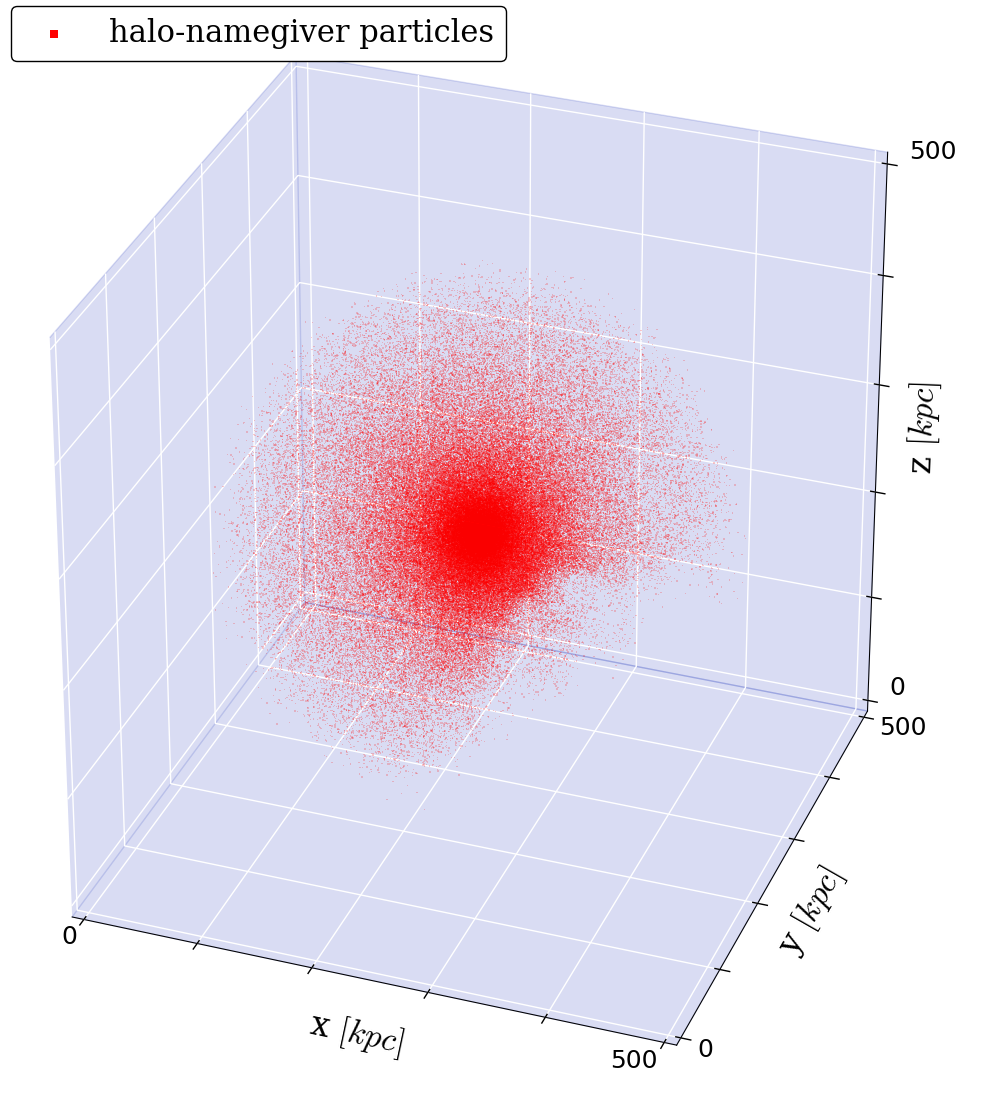
\includegraphics[width = .49\textwidth]{../report/images/dice-two/dice-two-halo-only-phew.png}} \hspace*{-1em} 	& 
		{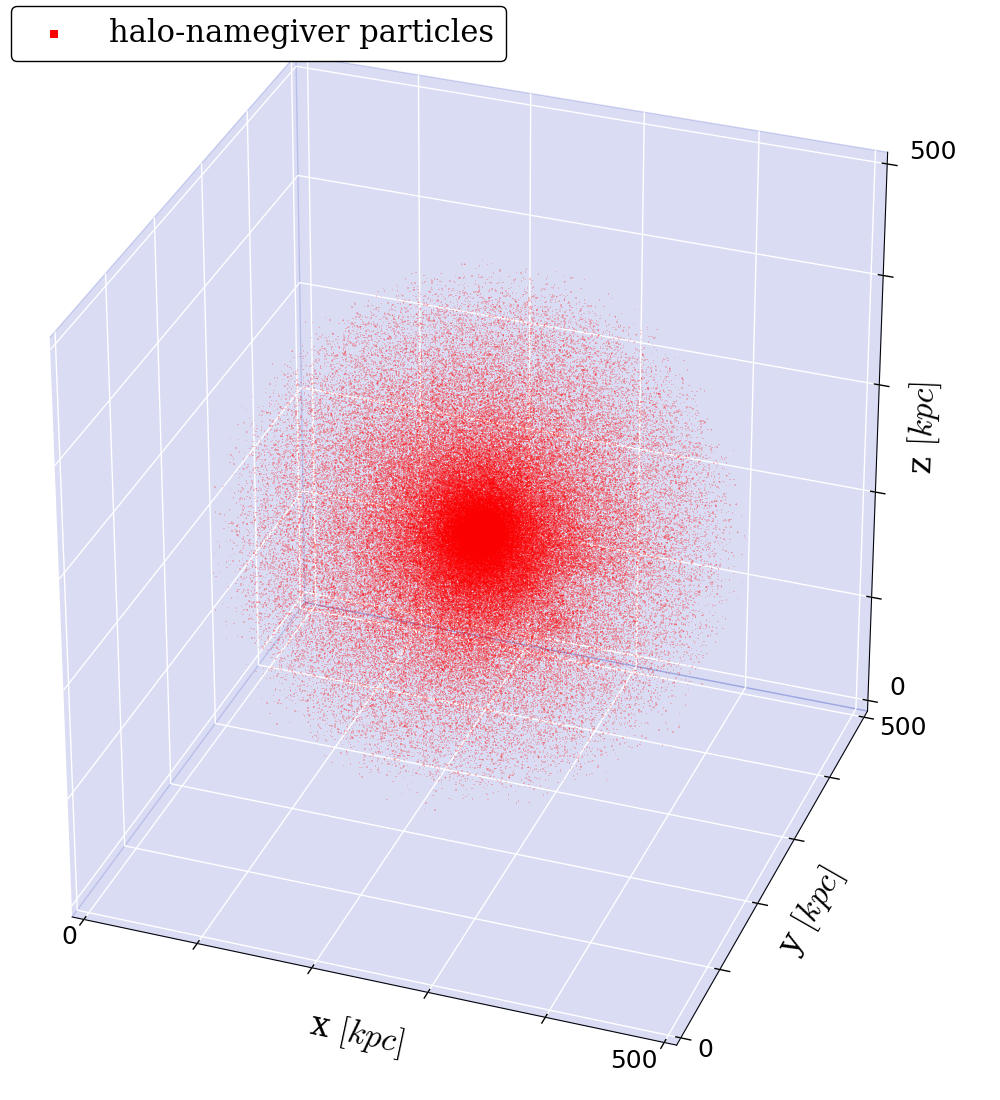
\includegraphics[width = .49\textwidth]{../report/images/dice-two/dice-two-halo-only-nosaddle.png}}
	\end{tabular}
\end{frame}




%\begin{frame}
%	\frametitle{Results: \ds-dataset}
%	
%	\begin{tabular}{c c}
%		\phewon\ 	& \simple \\[1.5em]
%		%
%		%	 
%		{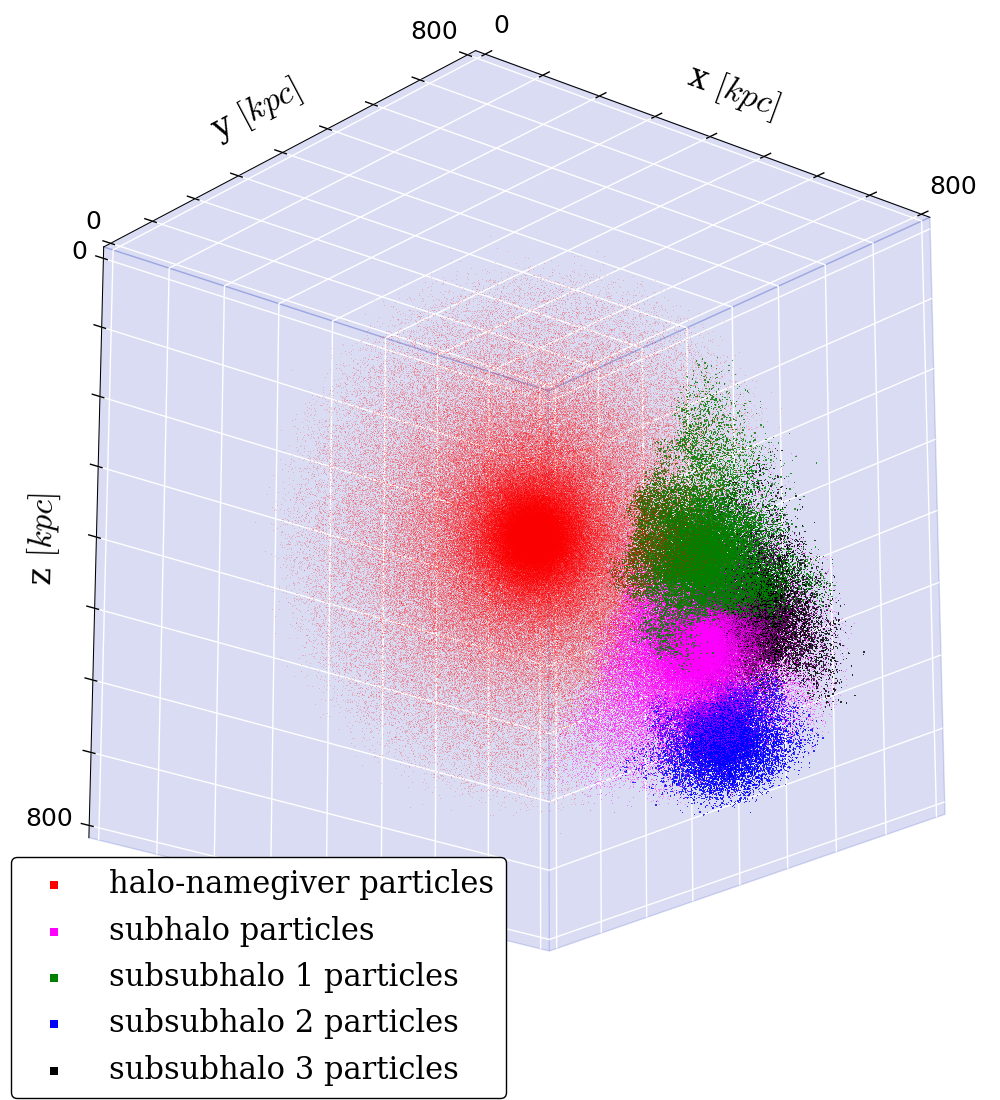
\includegraphics[width = .49\textwidth]{../report/images/dice-sub/dice-sub-plot-halo1-phew.png}} \hspace*{-1em} 	& 
%		{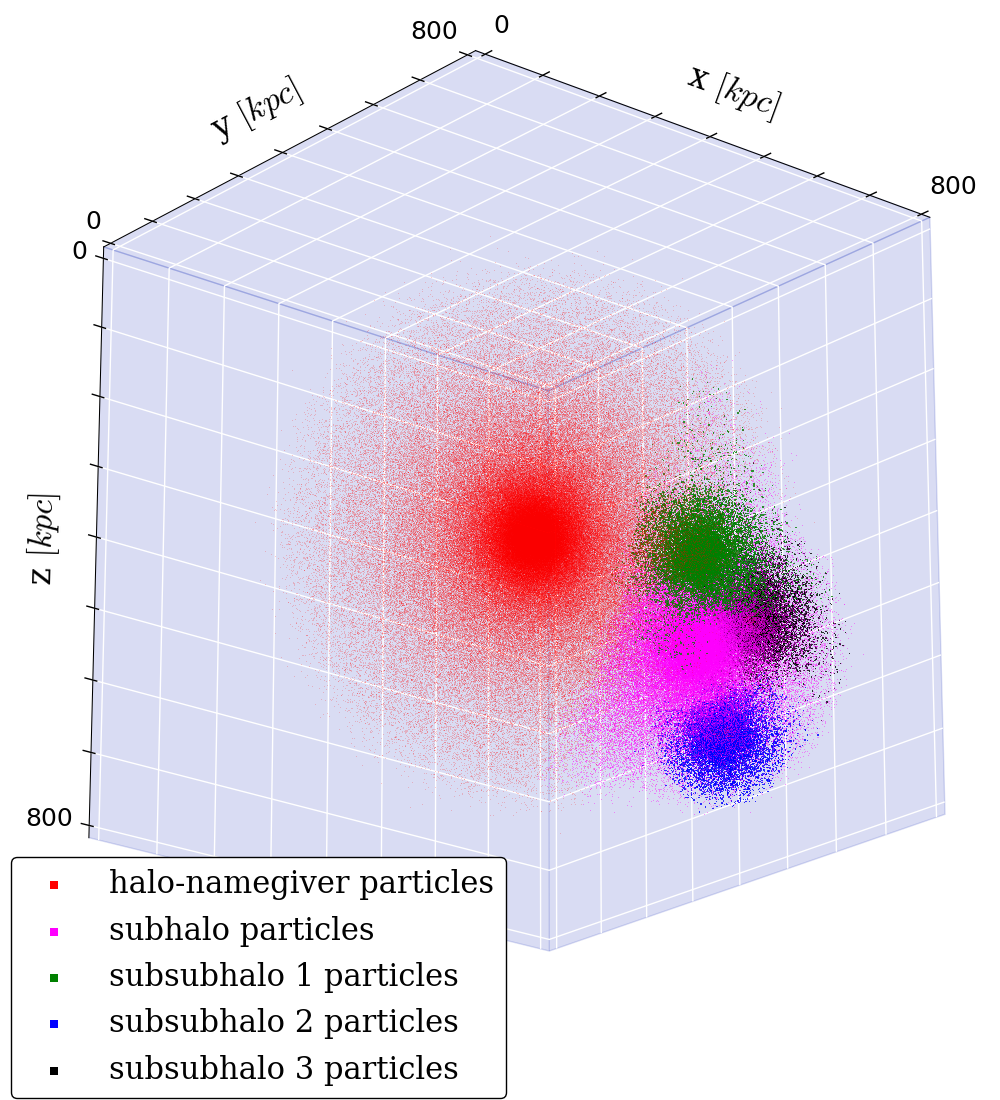
\includegraphics[width = .49\textwidth]{../report/images/dice-sub/dice-sub-plot-halo1-nosaddle.png}}
%	\end{tabular}
%\end{frame}
%
%
%
%\begin{frame}
%	\frametitle{Results: \ds-dataset: halo-namegiver particles only}
%	
%	\begin{tabular}{c c}
%		\phewon\ 	& \simple \\[1.5em]
%		%
%		%	 
%		{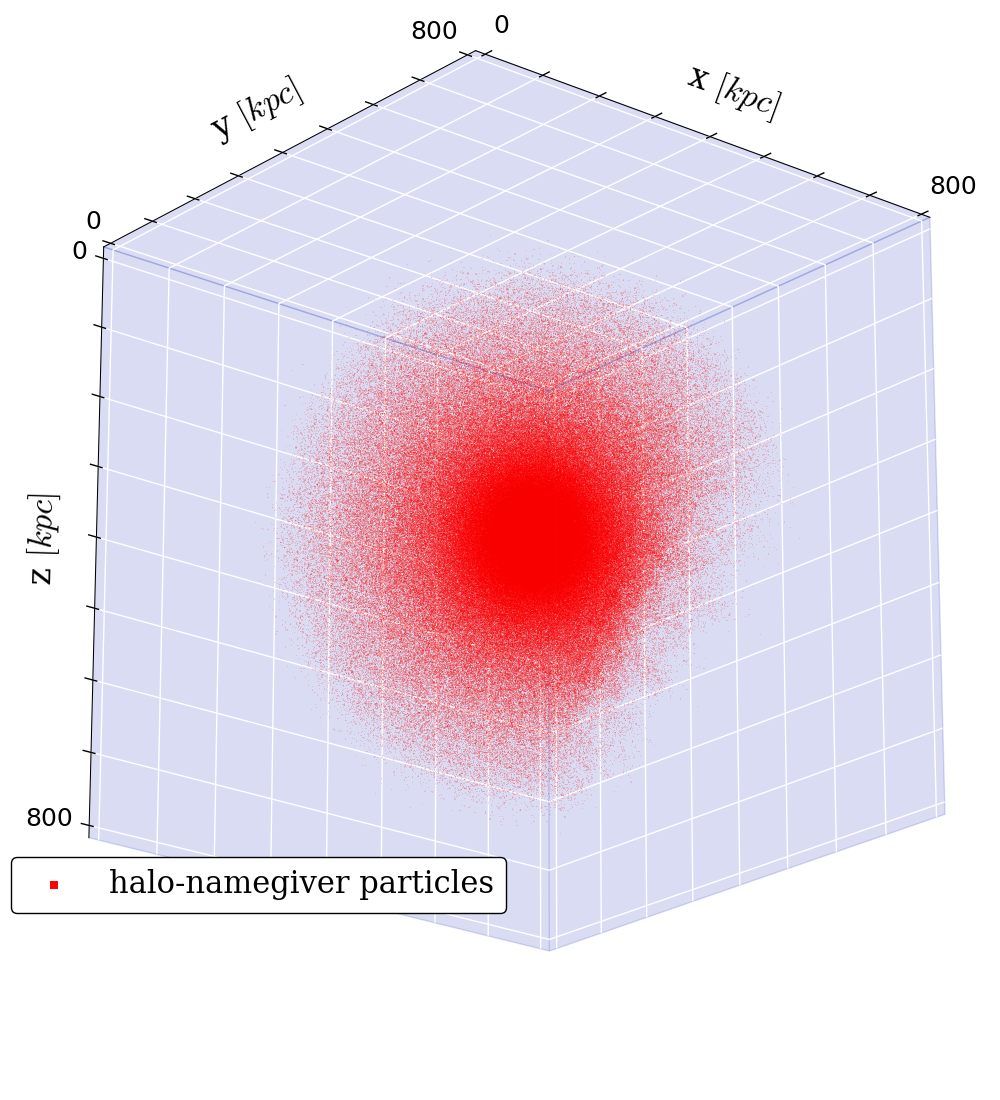
\includegraphics[width = .49\textwidth]{../report/images/dice-sub/dice-sub-halo-only-phew.png}} \hspace*{-1em} 	& 
%		{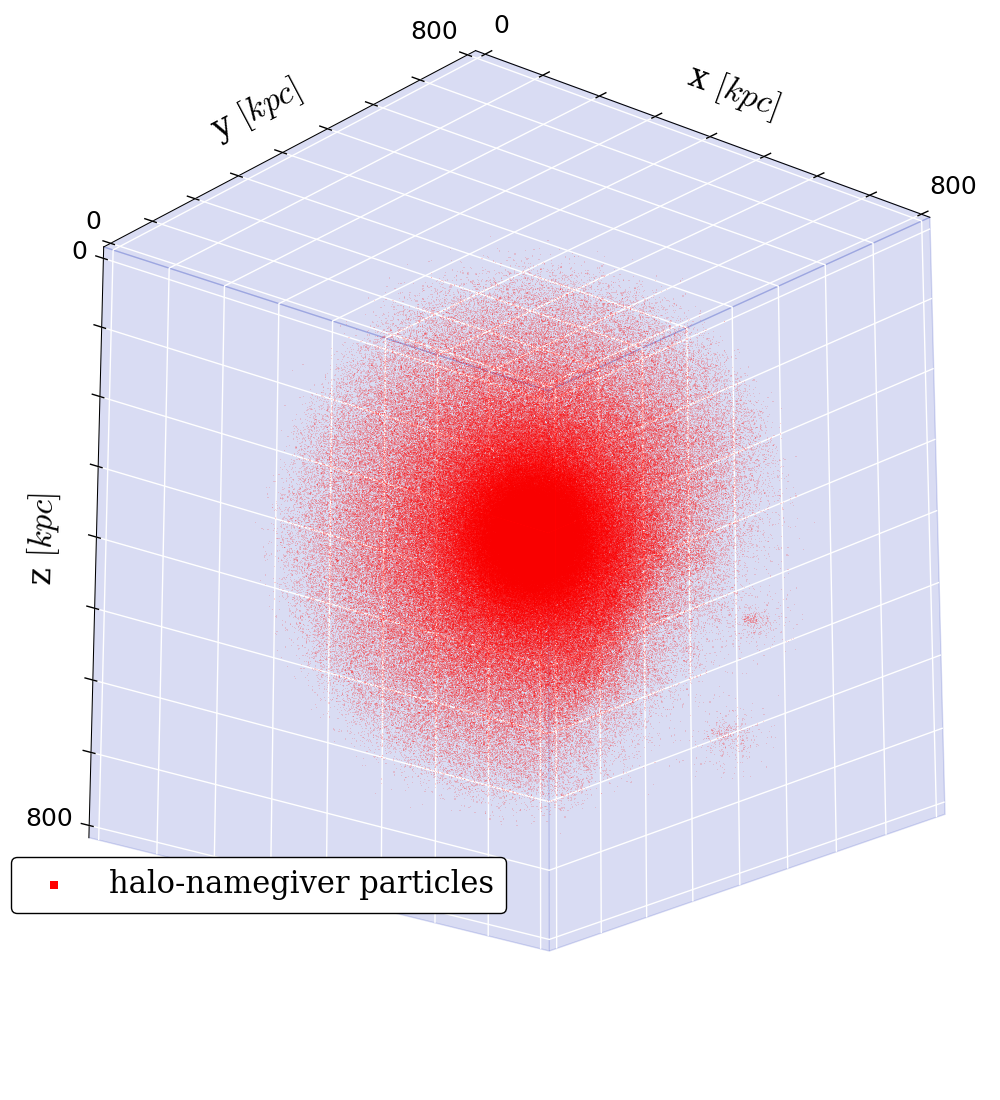
\includegraphics[width = .49\textwidth]{../report/images/dice-sub/dice-sub-halo-only-nosaddle.png}}
%	\end{tabular}
%\end{frame}



\begin{frame}
	\frametitle{Results: \cosmo-dataset: halo-namegiver particles only}
	
	\begin{tabular}{c c}
		\phewon\ 	& \simple \\[1.5em]
		%
		%	 
		{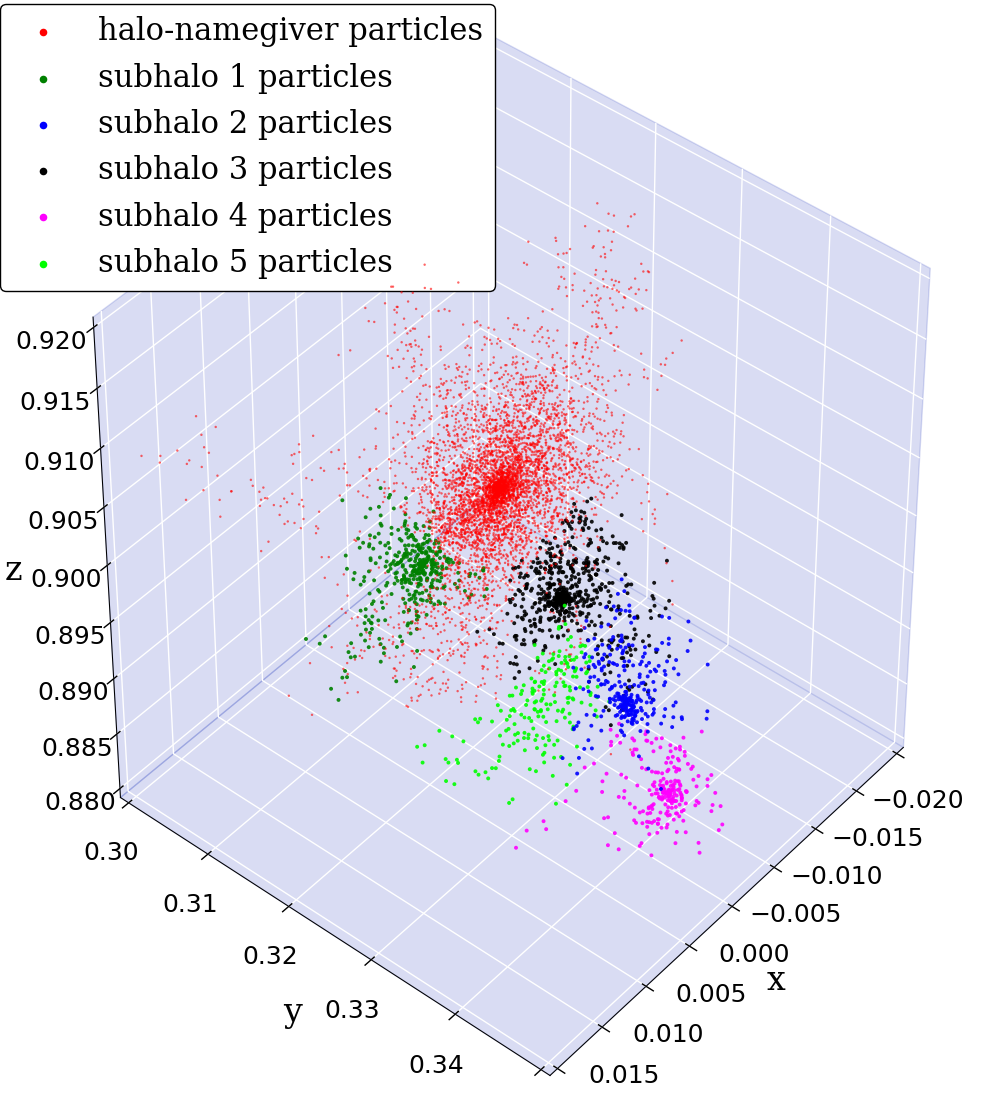
\includegraphics[width = .49\textwidth]{../report/images/cosmo/cos-halo-66858-phew.png}} \hspace*{-1em} 	& 
		{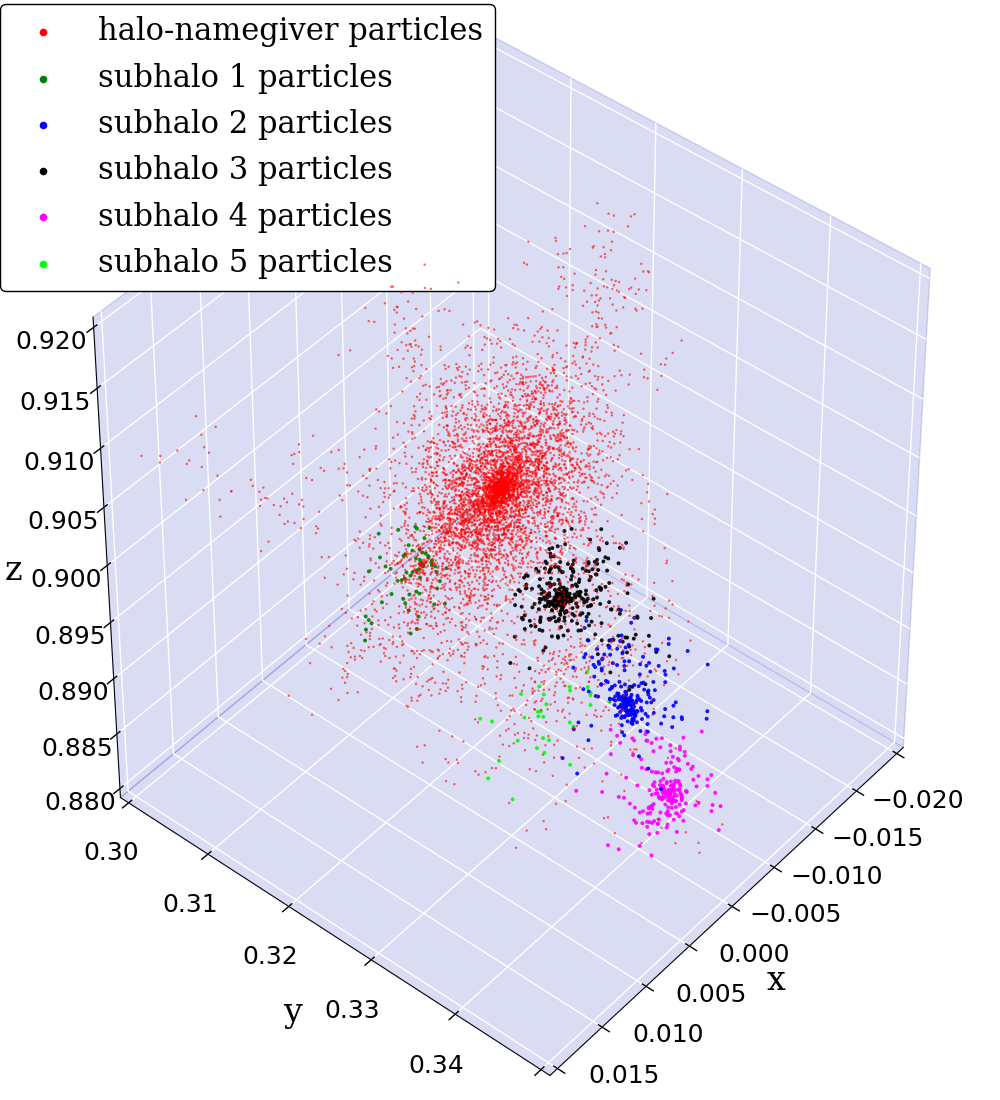
\includegraphics[width = .49\textwidth]{../report/images/cosmo/cos-halo-66858-nosaddle.png}}
	\end{tabular}
\end{frame}



\begin{frame}
	\frametitle{Results: \cosmo-dataset: halo-namegiver particles only}
	
	\begin{tabular}{c c}
		\phewon\ 	& \simple \\[1.5em]
		%
		%	 
		{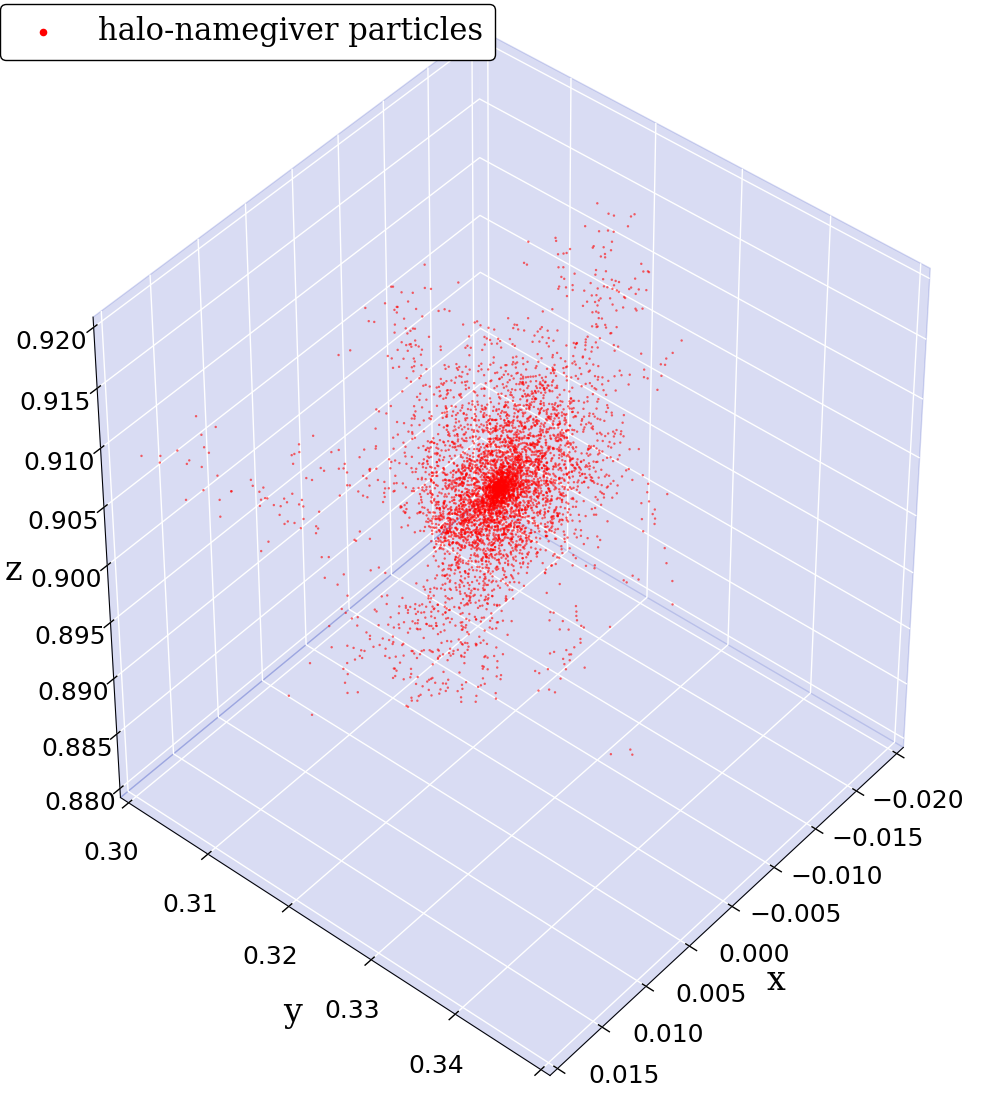
\includegraphics[width = .49\textwidth]{../report/images/cosmo/cos-halo-66858-halo-only-phew.png}} \hspace*{-1em} 	& 
		{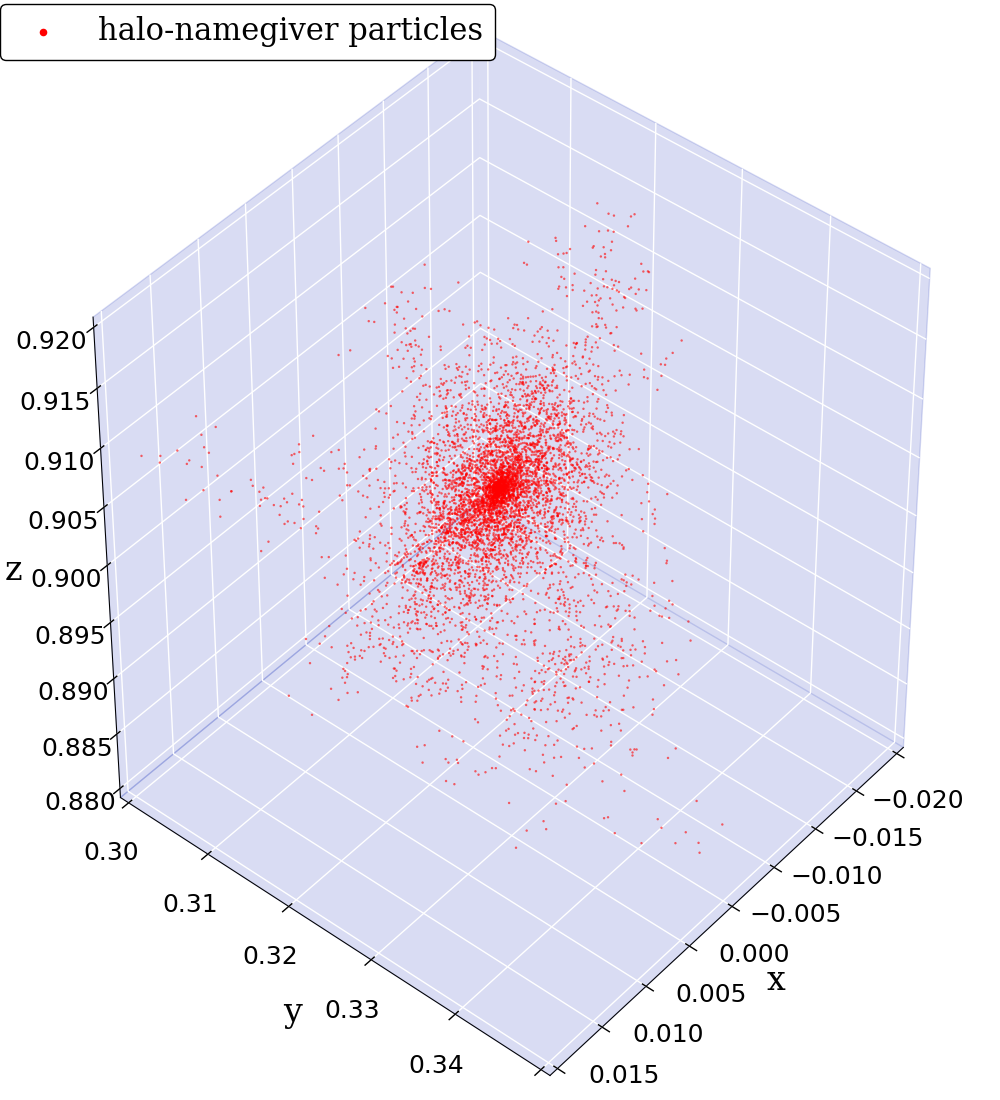
\includegraphics[width = .49\textwidth]{../report/images/cosmo/cos-halo-66858-halo-only-nosaddle.png}}
	\end{tabular}
\end{frame}